\documentclass[aspectratio=169,11pt,t,envcountsect,professionalfonts]{beamer}
\usepackage[main=polish,shorthands=off]{babel}
\usepackage{amsmath}
\usepackage{amssymb}
\usepackage{amsthm}
\usepackage{amsfonts}
\usepackage{xcolor}
\usepackage[utf8]{inputenc}
\usepackage[T1]{fontenc}
\usepackage{tikz}
\usetikzlibrary{patterns,decorations.pathreplacing,calc}


\makeatletter
\def\input@path{{styles/}}
\makeatother


\usepackage[autostyle]{csquotes}
\usepackage[
  backend=biber,
  style=numeric,
  maxbibnames=3,
  giveninits=true,
  doi=false,
  isbn=false,
  url=false,
]{biblatex}
\addbibresource{refs.bib}
\renewcommand*{\bibfont}{\footnotesize}

\input{macros}

\graphicspath{{figures/}}

% The optional argument is the short title used in the footline.
\title[Miara Lebesgue'a w $\mathbb{R}^n$]{Konstrukcja miary Lebesgue'a w $\mathbb{R}^n$}
\subtitle{Charakteryzacja zbiorów mierzalnych i własności miary}
\author{Tomasz Perek}
\institute{Matematyka zaoczna III rok\\ UKSW}
\date{\today}

\begin{document}

\begin{frame}[plain,t,noframenumbering]
  \titlepage
\end{frame}

% ======================================================================
\section{Wstęp}
% ======================================================================

\begin{frame}{Problem miary}
  Szukamy funkcji $\mu$ przypisującej podzbiorom $\R$ (ogólniej $\Rn$) ich „wielkość”, takiej że:
  \begin{enumerate}
    \item[(0)] $\mu(\emptyset) = 0$ oraz $\mu\big(\bigcup_j A_j\big) = \sum_j \mu(A_j)$ dla parami rozłącznych $A_j$ ($\sigma$-addytywność),
    \item[(1)] $\mu$ jest określona na \textbf{wszystkich} podzbiorach $\R$,
    \item[(2)] $\mu$ jest \textbf{niezmiennicza na przesunięcia}: $\mu(x + A) = \mu(A)$,
    \item[(3)] $\mu([0,1]) = 1$.
  \end{enumerate}

  \medskip
  \begin{block}{Odpowiedź (Vitali, 1905)}
    Przy aksjomacie wyboru taka miara \textbf{nie istnieje}.
  \end{block}

  \medskip
  Miara Lebesgue'a spełnia (0), (2), (3), a zamiast (1) dzieli podzbiory na \textbf{mierzalne} i \textbf{niemierzalne}.
\end{frame}

\begin{frame}{Plan konstrukcji}
  \begin{center}
  \begin{tikzpicture}[
      box/.style={draw, rounded corners, fill=blue!8, minimum width=2.8cm, minimum height=1.0cm, align=center, font=\small},
      arr/.style={-latex, thick}]
    \node[box] (V) at (0,0) {objętość kostki\\ $V^n(P)$};
    \node[box] (L) at (3.7,0) {miara zewnętrzna\\ $\lzn$ na $\Pow(\Rn)$};
    \node[box] (C) at (7.4,0) {warunek\\ Carathéodory'ego};
    \node[box] (M) at (11.1,0) {miara Lebesgue'a\\ $\lambda^n$ na $\LRn$};
    \draw[arr] (V) -- (L);
    \draw[arr] (L) -- (C);
    \draw[arr] (C) -- (M);
  \end{tikzpicture}
  \end{center}

  \begin{itemize}
    \item Rozdz.~2: rodziny zbiorów, kostki, zbiory borelowskie
    \item Rozdz.~3: zewnętrzna miara Lebesgue'a $\lzn$
    \item Rozdz.~4: konstrukcja Carathéodory'ego, $\BorelRn \subseteq \LRn$
    \item Rozdz.~5: charakteryzacja zbiorów mierzalnych, zbiór Vitalego
    \item Rozdz.~6: własności miary: jednoznaczność, geometria, bezatomowość
  \end{itemize}
\end{frame}

% ======================================================================
\section{Podstawowe pojęcia}
% ======================================================================

\begin{frame}{Rodziny zbiorów}
  \begin{mydef}[$\sigma$-algebra]
    Rodzinę $\mathcal{M} \subseteq \Pow(X)$ nazywamy \textbf{$\sigma$-algebrą}, jeżeli
    $X \in \mathcal{M}$, $A \in \mathcal{M} \Rightarrow X \setminus A \in \mathcal{M}$ oraz
    $A_1, A_2, \ldots \in \mathcal{M} \Rightarrow \bigcup_{j} A_j \in \mathcal{M}$.
  \end{mydef}
  \textit{Algebra}: to samo, ale tylko dla sum skończonych.

  \begin{mydef}[Zbiory borelowskie]
    $\BorelRn$ to najmniejsza $\sigma$-algebra zawierająca wszystkie zbiory otwarte w $\Rn$.
  \end{mydef}

  \begin{mydef}[Klasy $G_\delta$ i $F_\sigma$]
    $G_\delta$: przeliczalne przekroje zbiorów otwartych, \quad
    $F_\sigma$: przeliczalne sumy zbiorów domkniętych.
  \end{mydef}
  Np.\ $\Q = \bigcup_{q \in \Q}\{q\}$ jest typu $F_\sigma$, a $\R \setminus \Q$ typu $G_\delta$.
\end{frame}

\begin{frame}{Kostki i ich objętość}
  \begin{columns}[T]
    \begin{column}{0.58\textwidth}
      \begin{mydef}[Kostka]
        \textbf{Kostką} w $\Rn$ nazywamy iloczyn kartezjański przedziałów
        \[
          P = I_1 \times I_2 \times \cdots \times I_n,
        \]
        gdzie $I_j$ ma końce $a_j < b_j$ (otwarty, domknięty lub półotwarty).
      \end{mydef}
      \begin{mydef}[Objętość elementarna]
        \[
          V^n(P) = \prod_{j=1}^{n} (b_j - a_j).
        \]
      \end{mydef}
    \end{column}
    \begin{column}{0.38\textwidth}
      \begin{center}
      \begin{tikzpicture}[scale=1.0]
        \draw[-latex] (-0.3,0) -- (3.4,0) node[below]{$x_1$};
        \draw[-latex] (0,-0.3) -- (0,2.7) node[left]{$x_2$};
        \fill[blue!15] (0.8,0.6) rectangle (2.9,2.0);
        \draw[thick, blue!70!black] (0.8,0.6) rectangle (2.9,2.0);
        \draw[dashed] (0.8,0.6) -- (0.8,0) node[below]{$a_1$};
        \draw[dashed] (2.9,0.6) -- (2.9,0) node[below]{$b_1$};
        \draw[dashed] (0.8,0.6) -- (0,0.6) node[left]{$a_2$};
        \draw[dashed] (0.8,2.0) -- (0,2.0) node[left]{$b_2$};
        \node at (1.85,1.3) {$P$};
        \node[font=\footnotesize, align=center] at (1.6,-0.95) {$V^2(P) = (b_1-a_1)(b_2-a_2)$};
      \end{tikzpicture}
      \end{center}
    \end{column}
  \end{columns}
\end{frame}

\begin{frame}{Quiz: podstawowe pojęcia}
  \begin{enumerate}
    \item Czy każda $\sigma$-algebra jest algebrą zbiorów?
    \item Czy zbiór liczb wymiernych $\Q$ jest typu $G_\delta$?
    \item Czy kostka otwarta $(0,1)^n$ i kostka domknięta $[0,1]^n$ mają tę samą objętość elementarną?
  \end{enumerate}
\end{frame}

\begin{frame}{Quiz: podstawowe pojęcia --- odpowiedzi}
  \begin{enumerate}
    \item \TAK{} --- zamkniętość na sumy przeliczalne daje w szczególności zamkniętość na sumy skończone.
    \item \NIE{} --- $\Q$ jest typu $F_\sigma$, a z twierdzenia Baire'a nie jest typu $G_\delta$.
    \item \TAK{} --- $V^n$ zależy tylko od długości krawędzi, a nie od tego, czy brzeg należy do kostki.
  \end{enumerate}
\end{frame}

% ======================================================================
\section{Zewnętrzna miara Lebesgue'a}
% ======================================================================

\begin{frame}{Miara zewnętrzna}
  \begin{mydef}[Miara zewnętrzna]
    Funkcję $\phi\colon \Pow(X) \to [0, +\infty]$ nazywamy \textbf{miarą zewnętrzną}, jeżeli:
    \begin{enumerate}
      \item $\phi(\emptyset) = 0$,
      \item $A \subseteq B \Rightarrow \phi(A) \le \phi(B)$ \hfill (monotoniczność)
      \item $\phi\big(\bigcup_j A_j\big) \le \sum_j \phi(A_j)$ \hfill (przeliczalna podaddytywność)
    \end{enumerate}
  \end{mydef}

  \begin{mydef}[Zewnętrzna miara Lebesgue'a]
    \[
      \lzn(A) := \inf \Big\{ \sum_{j=1}^\infty V^n(P_j) \colon P_j \text{ -- kostki domknięte},\ A \subseteq \bigcup_{j=1}^\infty P_j \Big\}.
    \]
  \end{mydef}
  Pokrycia są \textbf{przeliczalne}, a nie skończone (jak w mierze Jordana).
\end{frame}

\begin{frame}{Idea: przybliżanie z zewnątrz}
  \begin{center}
    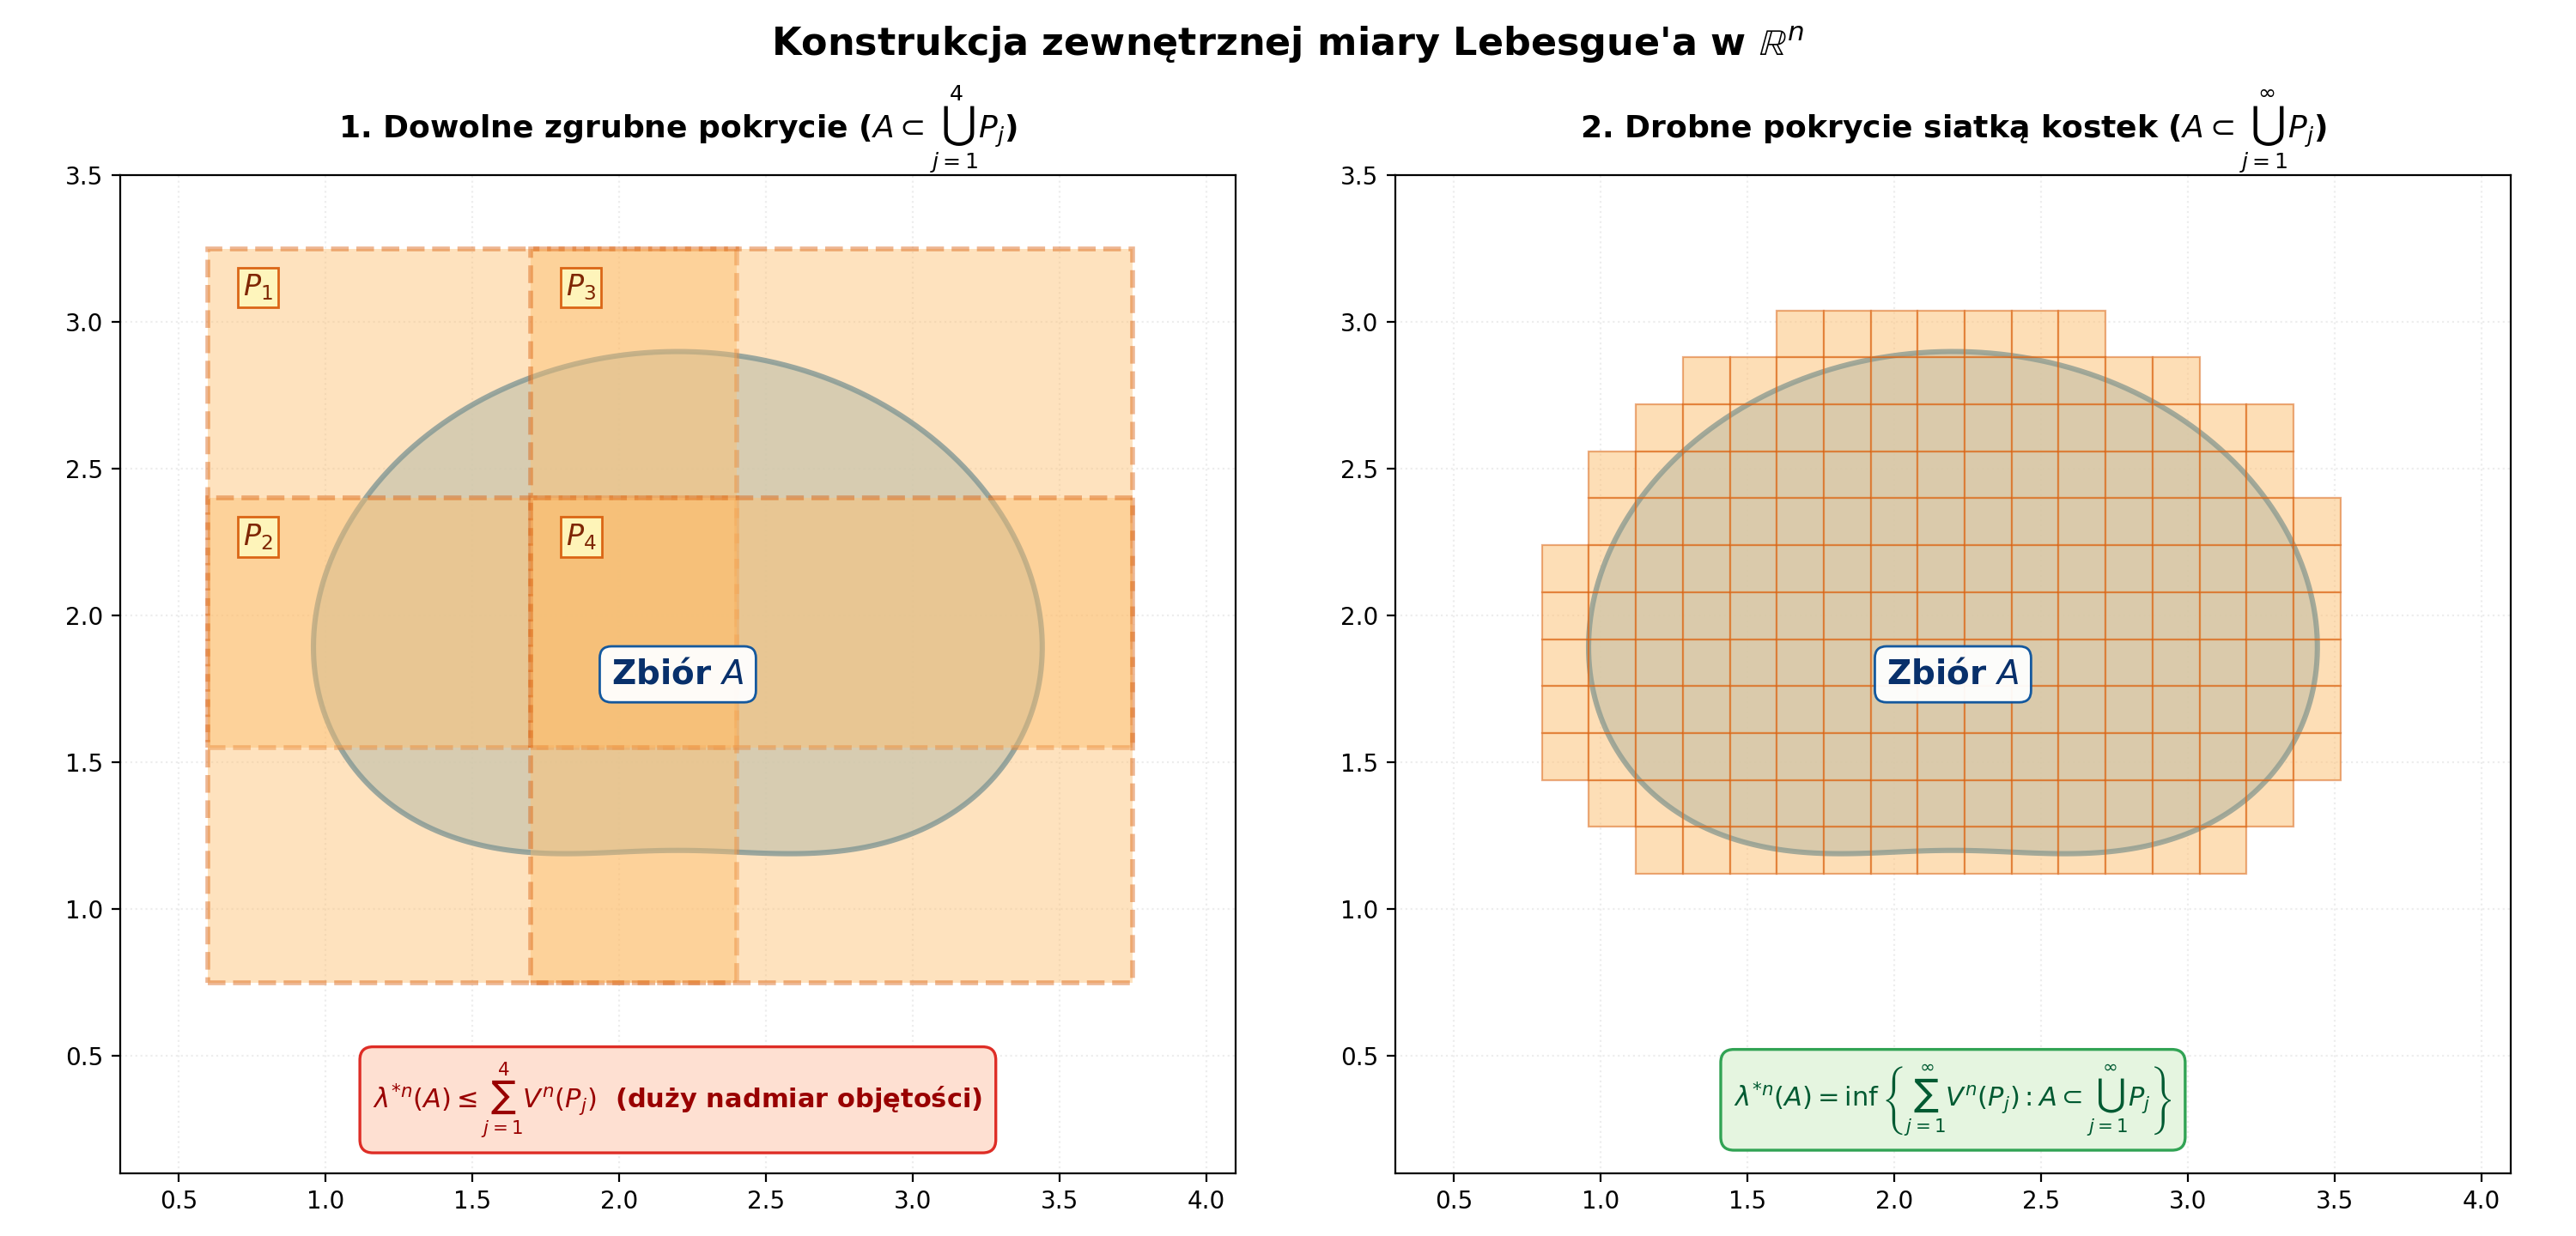
\includegraphics[height=0.62\textheight]{miara_zewnetrzna_v4.png}
  \end{center}
  Zgrubne pokrycie kostkami daje nadmiar; infimum po coraz drobniejszych pokryciach daje $\lzn(A)$.
\end{frame}

\begin{frame}{Zgodność z objętością i własności $\lzn$}
  \begin{mythm}[Objętość kostki]
    Dla dowolnej kostki $P \subseteq \Rn$: \quad $\lzn(P) = V^n(P)$.
  \end{mythm}
  \textit{Idea:} „$\le$” --- $P$ pokrywa samą siebie; „$\ge$” --- zwartość $\overline{P}$ pozwala przejść do skończonego pokrycia i porównać objętości.

  \begin{mythm}[Własności $\lzn$]
    \begin{enumerate}
      \item $\lzn$ jest miarą zewnętrzną;
      \item zbiory przeliczalne mają miarę zero, zbiory ograniczone --- skończoną;
      \item $\lzn(x_0 + A) = \lzn(A)$ \quad oraz \quad $\lzn(sA) = |s|^n \lzn(A)$;
      \item dla każdego $Y \subseteq \Rn$ istnieje $G \supseteq Y$ typu $G_\delta$ z $\lzn(G) = \lzn(Y)$.
    \end{enumerate}
  \end{mythm}
\end{frame}

\begin{frame}{Quiz: miara zewnętrzna}
  \begin{enumerate}
    \item Czy $\lzn$ jest przeliczalnie addytywna na wszystkich podzbiorach $\Rn$?
    \item Czy $\lambda^{*1}(\Q \cap [0,1]) = 0$?
    \item Czy w definicji $\lzn$ można ograniczyć się do pokryć \textbf{skończonych} i otrzymać tę samą funkcję?
  \end{enumerate}
\end{frame}

\begin{frame}{Quiz: miara zewnętrzna --- odpowiedzi}
  \begin{enumerate}
    \item \NIE{} --- jest tylko przeliczalnie podaddytywna; zbiór Vitalego pokaże, że addytywność może zawodzić.
    \item \TAK{} --- $j$-tą liczbę wymierną pokrywamy przedziałem długości $\eps 2^{-j}$, co daje sumę $\le \eps$.
    \item \NIE{} --- dla $\Q \cap [0,1]$ pokrycia skończone dają zawsze sumę $\ge 1$ (zewnętrzna miara Jordana).
  \end{enumerate}
\end{frame}

% ======================================================================
\section{Konstrukcja Carathéodory'ego}
% ======================================================================

\begin{frame}{Warunek Carathéodory'ego}
  \begin{columns}[T]
    \begin{column}{0.56\textwidth}
      \begin{mydef}[Zbiór $\phi$-mierzalny]
        $A \subseteq X$ jest \textbf{mierzalny w sensie Carathéodory'ego}, jeżeli dla każdego zbioru testowego $T \subseteq X$:
        \[
          \phi(T) = \phi(T \cap A) + \phi(T \setminus A).
        \]
      \end{mydef}
      Nierówność „$\le$” zachodzi zawsze (podaddytywność), więc sprawdzamy tylko „$\ge$”.

      \medskip
      Intuicja: $A$ „tnie” każdy zbiór $T$ czysto, bez straty ani nadmiaru miary.
    \end{column}
    \begin{column}{0.40\textwidth}
      \begin{center}
      \begin{tikzpicture}[scale=1.0]
        \begin{scope}
          \clip (0,0) ellipse (2.0 and 1.2);
          \fill[orange!35] (1.0,0) circle (1.3);
        \end{scope}
        \begin{scope}[even odd rule]
          \clip (0,0) ellipse (2.0 and 1.2) (1.0,0) circle (1.3);
          \fill[blue!15] (0,0) ellipse (2.0 and 1.2);
        \end{scope}
        \draw[thick, blue!70!black] (0,0) ellipse (2.0 and 1.2);
        \draw[thick, orange!80!black] (1.0,0) circle (1.3);
        \node at (-1.0,0) {$T \setminus A$};
        \node at (1.15,0) {$T \cap A$};
        \node[blue!70!black] at (-1.6,1.2) {$T$};
        \node[orange!80!black] at (2.45,0.95) {$A$};
      \end{tikzpicture}
      \end{center}
    \end{column}
  \end{columns}
\end{frame}

\begin{frame}{Twierdzenie Carathéodory'ego}
  \begin{mythm}[Carathéodory]
    Niech $\phi$ będzie miarą zewnętrzną na $X$, a $\mathcal{M}_\phi$ rodziną zbiorów $\phi$-mierzalnych. Wówczas:
    \begin{enumerate}
      \item $\mathcal{M}_\phi$ jest $\sigma$-algebrą;
      \item $\phi|_{\mathcal{M}_\phi}$ jest miarą (przeliczalnie addytywną);
      \item miara $\phi|_{\mathcal{M}_\phi}$ jest zupełna: $\phi(Z) = 0 \Rightarrow Z \in \mathcal{M}_\phi$.
    \end{enumerate}
  \end{mythm}

  \textit{Szkic dowodu:}
  \begin{itemize}
    \item warunek jest symetryczny względem $A \leftrightarrow X \setminus A$, więc $\mathcal{M}_\phi$ jest zamknięta na dopełnienia;
    \item dla dwóch zbiorów sprawdza się warunek, rozcinając $T$ na cztery części; stąd algebra;
    \item dla sum przeliczalnych rozłącznych: indukcja daje $\phi(T) \ge \sum_{j\le k} \phi(T \cap A_j) + \phi(T \setminus \bigcup_j A_j)$, potem $k \to \infty$.
  \end{itemize}
\end{frame}

\begin{frame}{Zbiory borelowskie są mierzalne}
  \begin{mydef}[Metryczna miara zewnętrzna]
    $\phi$ jest \textbf{metryczna}, gdy $\dist(A,B) > 0 \Rightarrow \phi(A \cup B) = \phi(A) + \phi(B)$.
  \end{mydef}

  \begin{mythm}
    \begin{enumerate}
      \item Dla metrycznej miary zewnętrznej każdy zbiór borelowski jest $\phi$-mierzalny.
      \item $\lzn$ jest metryczna.
    \end{enumerate}
  \end{mythm}

  \textit{Dowód (2):} pokrywamy $A \cup B$ kostkami o średnicy $< \dist(A,B)/3$. Żadna kostka nie trafia jednocześnie w $A$ i $B$, więc pokrycie rozpada się na pokrycie $A$ i pokrycie $B$: $\lzn(A) + \lzn(B) \le \lzn(A \cup B) + \eps$.

  \begin{mydef}[Miara Lebesgue'a]
    $\LRn := \mathcal{M}_{\lzn}$, \quad $\lambda^n := \lzn|_{\LRn}$. \quad Zatem $\BorelRn \subseteq \LRn$.
  \end{mydef}
\end{frame}

\begin{frame}{Quiz: konstrukcja Carathéodory'ego}
  \begin{enumerate}
    \item Czy zbiór $Z$ o mierze zewnętrznej $\lzn(Z) = 0$ jest mierzalny w sensie Lebesgue'a?
    \item Czy do sprawdzenia warunku Carathéodory'ego wystarczy nierówność $\phi(T) \ge \phi(T \cap A) + \phi(T \setminus A)$?
    \item Czy każdy zbiór domknięty w $\Rn$ jest mierzalny w sensie Lebesgue'a?
  \end{enumerate}
\end{frame}

\begin{frame}{Quiz: konstrukcja Carathéodory'ego --- odpowiedzi}
  \begin{enumerate}
    \item \TAK{} --- $\lzn(T \cap Z) = 0$ i $\lzn(T \setminus Z) \le \lzn(T)$, więc warunek zachodzi.
    \item \TAK{} --- nierówność przeciwna wynika zawsze z podaddytywności miary zewnętrznej.
    \item \TAK{} --- zbiór domknięty jest borelowski, a $\BorelRn \subseteq \LRn$.
  \end{enumerate}
\end{frame}

% ======================================================================
\section{Charakteryzacja zbiorów mierzalnych}
% ======================================================================

\begin{frame}{Podstawowe własności $\LRn$}
  \begin{mythm}
    \begin{enumerate}
      \item $\LRn$ jest $\sigma$-algebrą (dopełnienia, sumy i przekroje przeliczalne, różnice);
      \item $\lambda^n$ jest zupełna: podzbiór zbioru miary zero jest mierzalny i ma miarę zero;
      \item każdy zbiór co najwyżej przeliczalny (np.\ $\Q^n$) ma miarę zero.
    \end{enumerate}
  \end{mythm}

  \begin{block}{Relacje z innymi klasami}
    \[
      \BorelRn \subsetneq \LRn \subsetneq \Pow(\Rn).
    \]
    Pierwsza inkluzja właściwa: zbiór Cantora; druga: zbiór Vitalego.
  \end{block}
\end{frame}

\begin{frame}{Topologiczna charakteryzacja mierzalności}
  \begin{columns}[T]
    \begin{column}{0.6\textwidth}
      \begin{mythm}
        Dla $A \subseteq \Rn$ równoważne są:
        \begin{enumerate}
          \item[(1)] $A \in \LRn$;
          \item[(2)] $\forall \eps > 0\ \exists G$ otwarty: $A \subseteq G$, $\lzn(G \setminus A) < \eps$;
          \item[(3)] $A = B \setminus C$, $B$ typu $G_\delta$, $\lambda^n(C) = 0$;
          \item[(4)] $\forall \eps > 0\ \exists F$ domknięty: $F \subseteq A$, $\lzn(A \setminus F) < \eps$;
          \item[(5)] $A = B \cup C$, $B$ typu $F_\sigma$, $\lambda^n(C) = 0$.
        \end{enumerate}
      \end{mythm}
      \small Zbiór mierzalny = zbiór borelowski „z dokładnością do zbioru miary zero”.
    \end{column}
    \begin{column}{0.37\textwidth}
      \begin{center}
      \begin{tikzpicture}[scale=0.95]
        \draw[thick, fill=blue!10, draw=blue!70!black]
          plot[smooth cycle, tension=0.8] coordinates {(-2.1,0) (-1.3,1.6) (0.4,1.9) (2.1,1.0) (2.0,-1.0) (0.3,-1.9) (-1.5,-1.4)};
        \draw[thick, fill=orange!25, draw=orange!80!black]
          plot[smooth cycle, tension=0.8] coordinates {(-1.7,0) (-1.0,1.25) (0.4,1.5) (1.7,0.8) (1.6,-0.8) (0.3,-1.5) (-1.2,-1.1)};
        \draw[thick, fill=green!20, draw=green!50!black, dashed]
          plot[smooth cycle, tension=0.8] coordinates {(-1.2,0) (-0.7,0.85) (0.4,1.05) (1.25,0.55) (1.15,-0.55) (0.3,-1.05) (-0.8,-0.75)};
        \node[blue!70!black] at (1.75,1.65) {$G$};
        \node[orange!80!black] at (1.35,-1.35) {$A$};
        \node[green!40!black] at (0.15,0) {$F$};
      \end{tikzpicture}

      \medskip
      {\small $F \subseteq A \subseteq G$,\\ $\lzn(G \setminus F) < 2\eps$}
      \end{center}
    \end{column}
  \end{columns}
\end{frame}

\begin{frame}{Regularność i uzupełnienie}
  \begin{mythm}[Regularność miary Lebesgue'a]
    Dla $A \in \LRn$:
    \[
      \lambda^n(A) = \inf\{\lambda^n(G)\colon G \supseteq A \text{ otwarty}\} = \sup\{\lambda^n(K)\colon K \subseteq A \text{ zwarty}\}.
    \]
  \end{mythm}

  \begin{mythm}[Struktura uzupełnienia]
    $\LRn$ jest uzupełnieniem $\BorelRn$ względem $\lambda^n$:
    \[
      \LRn = \{ B \cup Z \colon B \in \BorelRn,\ Z \subseteq N \text{ dla pewnego } N \in \BorelRn,\ \lambda^n(N) = 0 \}.
    \]
  \end{mythm}
  \textit{Idea:} z warunku (5) $A = B \cup C$, a zbiór $C$ miary zero mieści się w zbiorze typu $G_\delta$ miary zero.
\end{frame}

\begin{frame}{Zbiór Cantora: mierzalny, ale nie zawsze borelowski}
  \begin{center}
  \begin{tikzpicture}[xscale=10, yscale=0.55]
    \draw[line width=3pt, blue!70!black] (0,0) -- (1,0);
    \draw[line width=3pt, blue!70!black] (0,-1) -- (1/3,-1) (2/3,-1) -- (1,-1);
    \foreach \s in {0,2/3} {
      \draw[line width=3pt, blue!70!black] (\s,-2) -- ({\s+1/9},-2) ({\s+2/9},-2) -- ({\s+1/3},-2);
    }
    \foreach \s in {0,2/9,2/3,8/9} {
      \draw[line width=3pt, blue!70!black] (\s,-3) -- ({\s+1/27},-3) ({\s+2/27},-3) -- ({\s+1/9},-3);
    }
    \node[left, font=\small] at (0,0) {$C_0$};
    \node[left, font=\small] at (0,-1) {$C_1$};
    \node[left, font=\small] at (0,-2) {$C_2$};
    \node[left, font=\small] at (0,-3) {$C_3$};
    \node[right, font=\small] at (1,0) {$1$};
    \node[right, font=\small] at (1,-1) {$2/3$};
    \node[right, font=\small] at (1,-2) {$(2/3)^2$};
    \node[right, font=\small] at (1,-3) {$(2/3)^3$};
  \end{tikzpicture}
  \end{center}

  \begin{itemize}
    \item $C = \bigcap_k C_k$ jest domknięty, $\lambda^1(C) \le (2/3)^k \to 0$, a mimo to $\#C = \mathfrak{c}$.
    \item Z zupełności każdy podzbiór $C$ jest mierzalny: $\#\LRn \ge \#\Pow(C) = 2^{\mathfrak{c}}$.
    \item Natomiast $\#\BorelRn = \mathfrak{c} < 2^{\mathfrak{c}}$, więc $\BorelRn \subsetneq \LRn$.
  \end{itemize}
\end{frame}

\begin{frame}{Zbiór Vitalego}
  \begin{mythm}[Vitali]
    Przy aksjomacie wyboru istnieje podzbiór $[0,1]$ niemierzalny w sensie Lebesgue'a.
  \end{mythm}
  \textit{Szkic:}
  \begin{itemize}
    \item $x \sim y \iff x - y \in \Q$; z aksjomatu wyboru bierzemy $V \subseteq [0,1]$ --- po jednym reprezentancie z każdej klasy.
    \item Dla wymiernych $r_k \in [-1,1]$ zbiory $V_k = V + r_k$ są parami rozłączne i
      \[
        [0,1] \subseteq \bigcup_{k} V_k \subseteq [-1,2].
      \]
    \item Gdyby $V$ był mierzalny, to $\lambda(V_k) = \lambda(V)$ i
      \[
        1 \le \sum_{k=1}^\infty \lambda(V) \le 3.
      \]
      Dla $\lambda(V) = 0$ suma to $0$, dla $\lambda(V) > 0$ suma to $\infty$ --- sprzeczność.
  \end{itemize}
\end{frame}

\begin{frame}{Quiz: charakteryzacja zbiorów mierzalnych}
  \begin{enumerate}
    \item Czy każdy zbiór mierzalny w sensie Lebesgue'a jest borelowski?
    \item Czy zbiór Cantora ma miarę zero, choć jest nieprzeliczalny?
    \item Czy zbiór niemierzalny da się skonstruować bez aksjomatu wyboru (w samym ZF)?
  \end{enumerate}
\end{frame}

\begin{frame}{Quiz: charakteryzacja zbiorów mierzalnych --- odpowiedzi}
  \begin{enumerate}
    \item \NIE{} --- zbiorów mierzalnych jest $2^{\mathfrak{c}}$ (podzbiory zbioru Cantora), a borelowskich tylko $\mathfrak{c}$.
    \item \TAK{} --- po $k$ krokach zostaje zbiór miary $(2/3)^k \to 0$, a $C$ ma moc continuum.
    \item \NIE{} --- Solovay (1970): przy założeniu istnienia liczby nieosiągalnej jest model ZF, w którym każdy podzbiór $\R$ jest mierzalny.
  \end{enumerate}
\end{frame}

% ======================================================================
\section{Własności miary Lebesgue'a}
% ======================================================================

\begin{frame}{Jednoznaczność miary Lebesgue'a}
  \begin{mythm}[Jednoznaczność przez objętość kostek]
    Jeśli $\mu$ jest miarą na $\LRn$ i $\mu(P) = V^n(P)$ dla każdej kostki domkniętej $P$, to $\mu = \lambda^n$.
  \end{mythm}

  \begin{mythm}[Jednoznaczność przez translacje]
    Jeśli $\mu$ jest miarą borelowską na $\Rn$, niezmienniczą na translacje i $\mu([0,1)^n) = 1$, to $\mu = \lambda^n$ na $\BorelRn$.
  \end{mythm}

  \textit{Idea:} $[0,1)^n$ dzieli się na $k^n$ przesuniętych kopii $[0,\frac1k)^n$, więc każda ma miarę $k^{-n}$. Stąd $\mu = \lambda^n$ na kostkach wymiernych, a te generują $\BorelRn$ (lemat Dynkina).
\end{frame}

\begin{frame}{Własności geometryczne}
  \begin{columns}[T]
    \begin{column}{0.48\textwidth}
      \begin{mythm}
        Dla $A \in \LRn$, $x_0 \in \Rn$, $s \in \R$:
        \begin{itemize}
          \item $\lambda^n(x_0 + A) = \lambda^n(A)$,
          \item $\lambda^n(sA) = |s|^n \lambda^n(A)$,
          \item $\lambda^n(T(A)) = |\det T|\, \lambda^n(A)$ \\ dla liniowego $T\colon \Rn \to \Rn$.
        \end{itemize}
      \end{mythm}
      \begin{mywn}
        Izometrie $\Phi(x) = Ox + x_0$ ($\det O = \pm 1$) zachowują miarę, np.\ obroty i symetrie.
      \end{mywn}
    \end{column}
    \begin{column}{0.5\textwidth}
      \begin{center}
        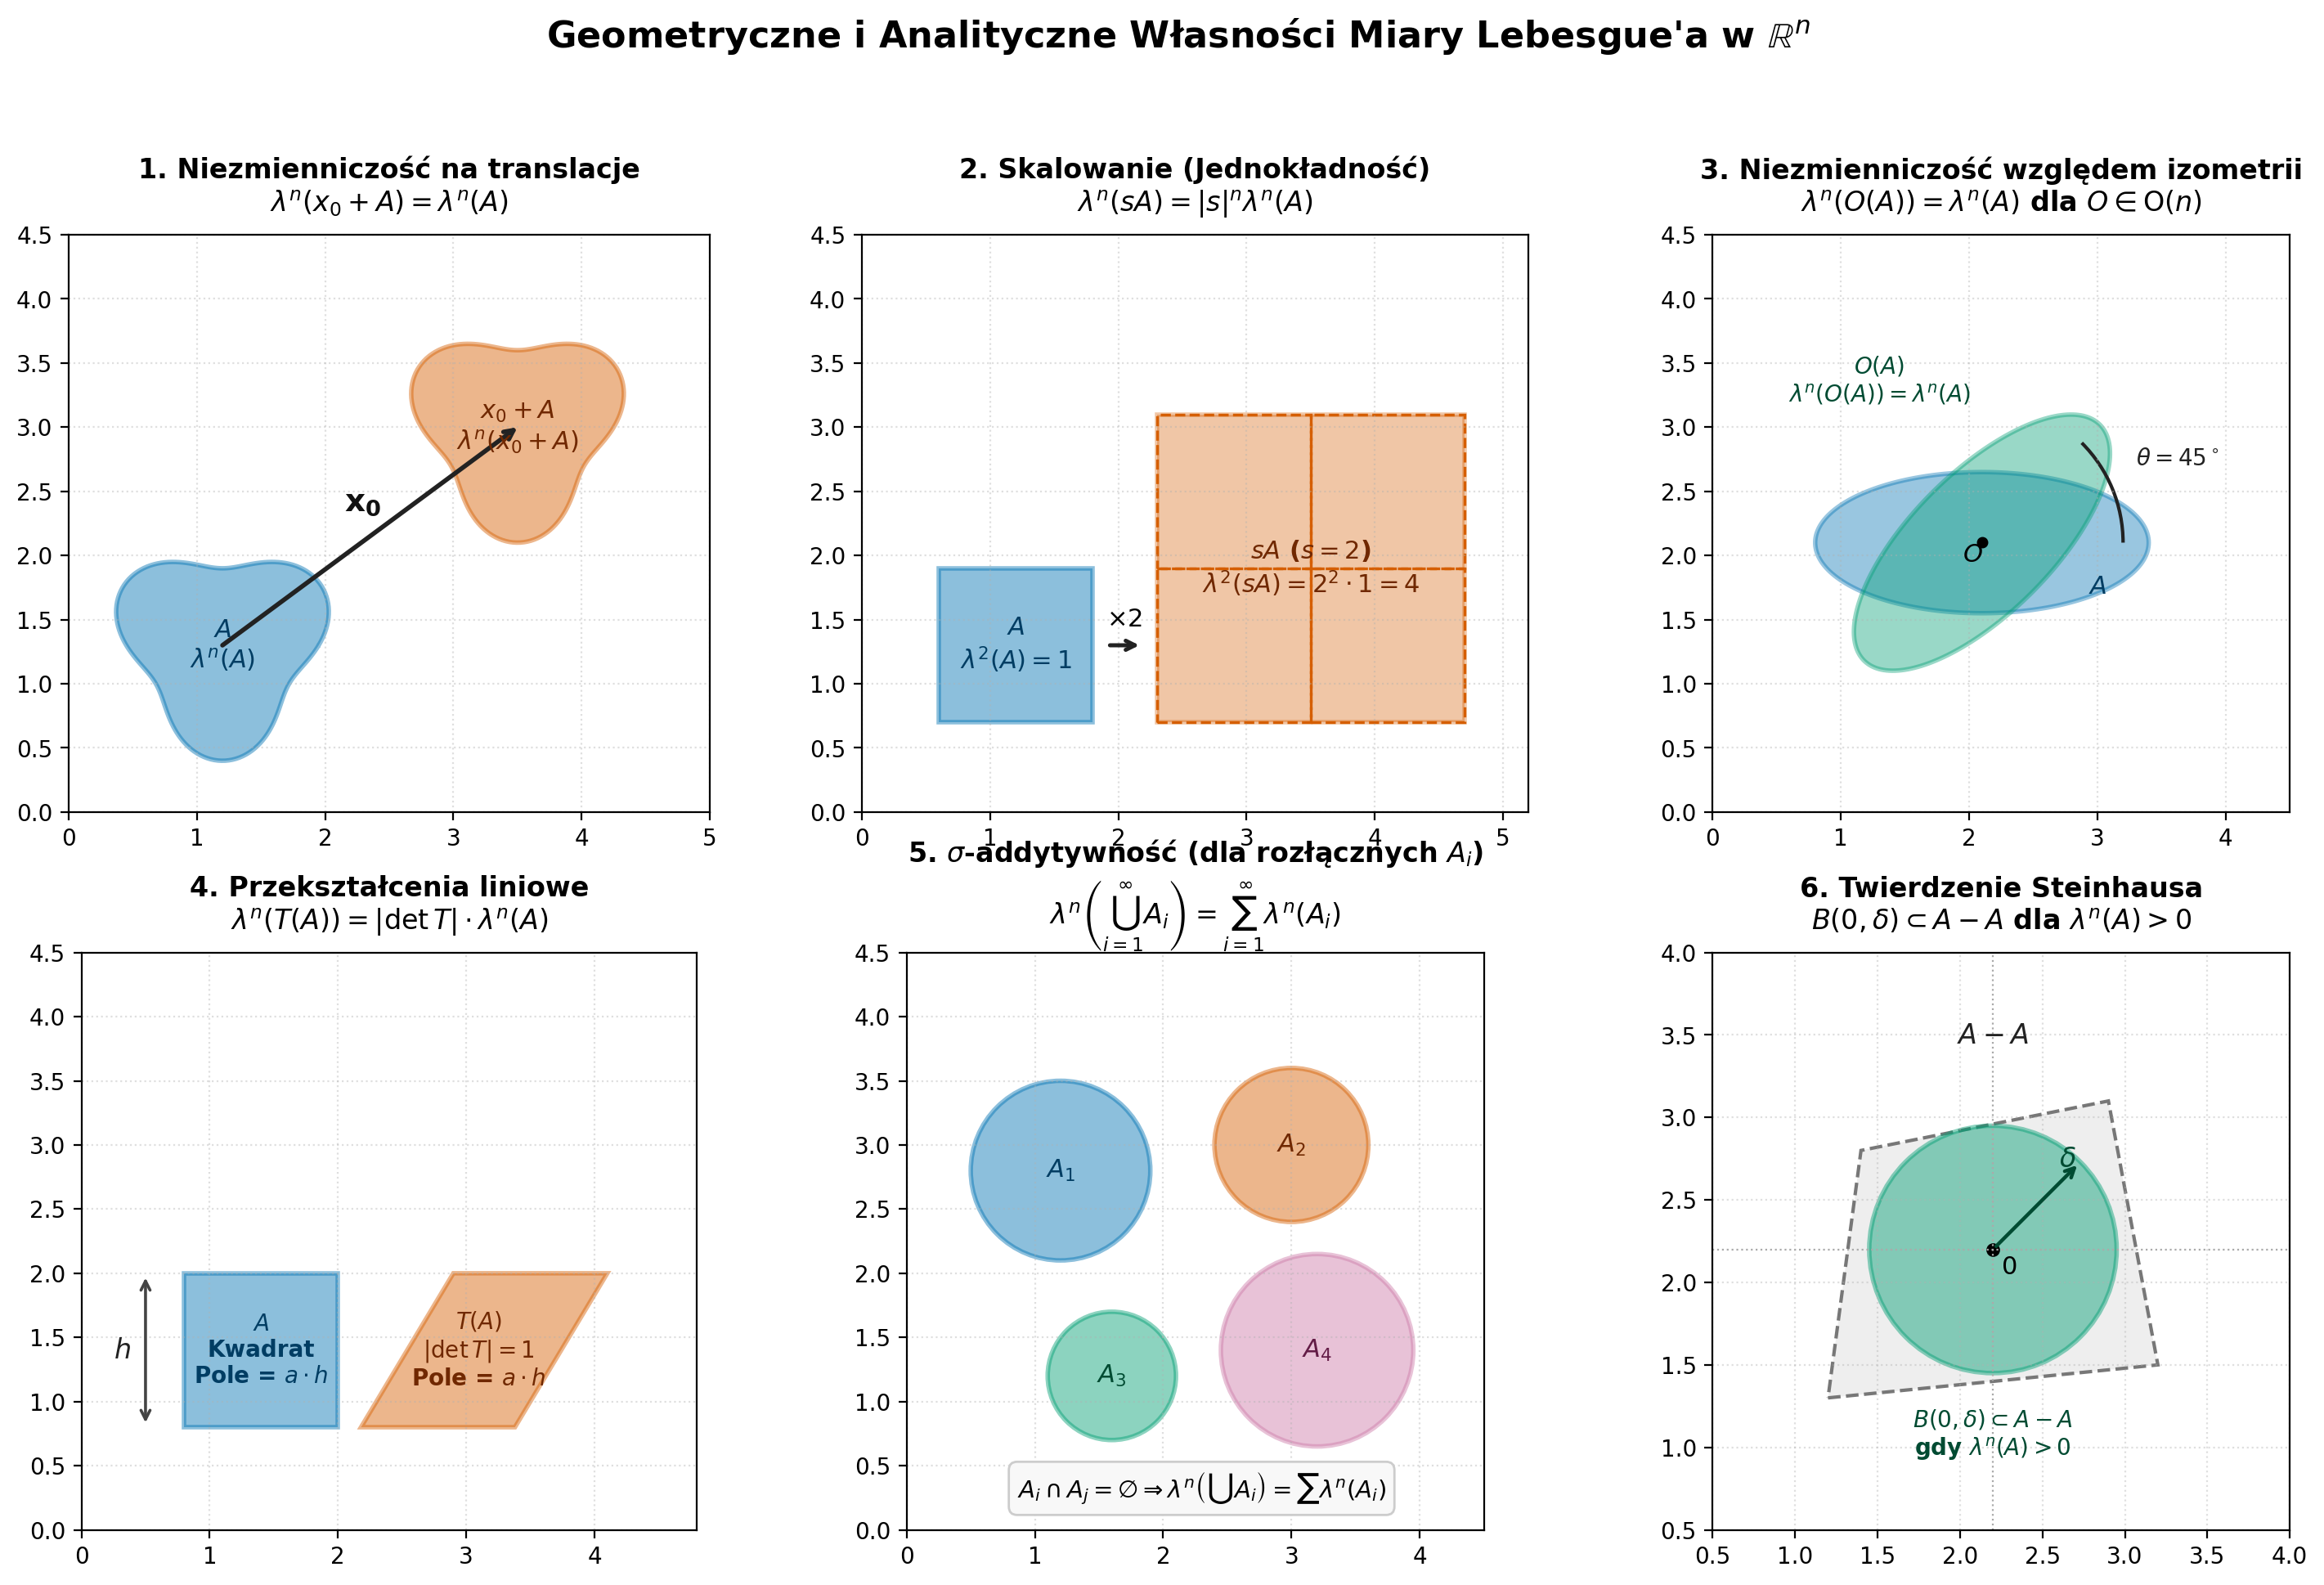
\includegraphics[width=\textwidth]{wlasnosci_miary_lebesguea.png}
      \end{center}
    \end{column}
  \end{columns}
\end{frame}

\begin{frame}{Skąd $|\det T|$? (dla $n = 2$)}
  \begin{center}
  \begin{tikzpicture}[scale=1.05]
    % skalowanie
    \begin{scope}
      \fill[blue!12] (0,0) rectangle (1,1); \draw[thick] (0,0) rectangle (1,1);
      \draw[-latex, thick] (1.2,0.5) -- (1.8,0.5);
      \fill[orange!25] (2,0) rectangle (3.6,0.7); \draw[thick] (2,0) rectangle (3.6,0.7);
      \node[font=\small, align=center] at (1.8,-0.6) {skalowanie $(ax, by)$\\ pole $\times |ab|$};
    \end{scope}
    % obrót
    \begin{scope}[xshift=4.4cm]
      \fill[blue!12] (0,0) rectangle (1,1); \draw[thick] (0,0) rectangle (1,1);
      \draw[-latex, thick] (1.2,0.5) -- (1.8,0.5);
      \begin{scope}[shift={(2.7,0)}, rotate=30]
        \fill[orange!25] (0,0) rectangle (1,1); \draw[thick] (0,0) rectangle (1,1);
      \end{scope}
      \node[font=\small, align=center] at (1.8,-0.6) {obrót\\ pole bez zmian};
    \end{scope}
    % ścinanie
    \begin{scope}[xshift=8.8cm]
      \fill[blue!12] (0,0) rectangle (1,1); \draw[thick] (0,0) rectangle (1,1);
      \draw[-latex, thick] (1.2,0.5) -- (1.8,0.5);
      \fill[orange!25] (2,0) -- (3,0) -- (3.6,1) -- (2.6,1) -- cycle;
      \draw[thick] (2,0) -- (3,0) -- (3.6,1) -- (2.6,1) -- cycle;
      \node[font=\small, align=center] at (1.8,-0.6) {ścinanie $(x+cy, y)$\\ pole bez zmian};
    \end{scope}
  \end{tikzpicture}
  \end{center}

  \begin{itemize}
    \item Każda odwracalna macierz $2 \times 2$ jest złożeniem skalowań, obrotów (symetrii) i ścinań.
    \item Wyznacznik złożenia to iloczyn wyznaczników, a pola mnożą się tak samo.
    \item Dla $\det T = 0$ obraz $T(\R^2)$ jest prostą lub punktem, czyli zbiorem miary zero.
  \end{itemize}
\end{frame}

\begin{frame}{Bezatomowość i własność Darboux}
  \begin{columns}[T]
    \begin{column}{0.58\textwidth}
      \begin{mythm}[Bezatomowość]
        Każdy zbiór $A \in \LRn$ z $\lambda^n(A) > 0$ zawiera mierzalny $B$ z $0 < \lambda^n(B) < \lambda^n(A)$.
      \end{mythm}
      \textit{Idea:} $f(t) = \lambda^n(A \cap \{x_1 \le t\})$ jest ciągła i rośnie od $0$ do $\lambda^n(A)$ (dla $A$ ograniczonego), więc przyjmuje wartość $\frac12 \lambda^n(A)$.

      \begin{mywn}[Własność Darboux]
        Dla $0 \le c \le \lambda^n(A)$ istnieje mierzalny $B \subseteq A$ z $\lambda^n(B) = c$.
      \end{mywn}
    \end{column}
    \begin{column}{0.4\textwidth}
      \begin{center}
      \begin{tikzpicture}[scale=0.95]
        \begin{scope}
          \clip plot[smooth cycle, tension=0.8] coordinates {(-1.8,0) (-1.1,1.3) (0.5,1.5) (1.9,0.6) (1.6,-1.0) (0.1,-1.5) (-1.3,-1.1)};
          \fill[orange!35] (-2.5,-2) rectangle (0.25,2);
          \fill[blue!10] (0.25,-2) rectangle (2.5,2);
        \end{scope}
        \draw[thick, blue!70!black] plot[smooth cycle, tension=0.8] coordinates {(-1.8,0) (-1.1,1.3) (0.5,1.5) (1.9,0.6) (1.6,-1.0) (0.1,-1.5) (-1.3,-1.1)};
        \draw[thick, red!70!black] (0.25,-1.9) -- (0.25,1.9) node[above]{$x_1 = t$};
        \draw[-latex] (-2.2,-2.1) -- (2.4,-2.1) node[below]{$x_1$};
        \node at (-0.8,0.1) {$f(t)$};
        \node[blue!70!black] at (1.75,1.25) {$A$};
      \end{tikzpicture}
      \end{center}
    \end{column}
  \end{columns}

  \smallskip
  \textbf{Steinhaus:} jeśli $\lambda^n(A) > 0$, to $A - A$ zawiera kulę $B(0,\delta)$. Daje to drugi dowód niemierzalności zbioru Vitalego, bo $(V - V) \cap \Q = \{0\}$.
\end{frame}

\begin{frame}{Quiz: własności miary Lebesgue'a}
  \begin{enumerate}
    \item Czy miara Lebesgue'a na płaszczyźnie jest niezmiennicza na obroty?
    \item Czy $\lambda^n$ ma atomy, czyli zbiory miary dodatniej bez podzbiorów o mniejszej dodatniej mierze?
    \item Czy dla przekształcenia liniowego $T$ z $\det T = -2$ zachodzi $\lambda^n(T(A)) = -2\,\lambda^n(A)$?
  \end{enumerate}
\end{frame}

\begin{frame}{Quiz: własności miary Lebesgue'a --- odpowiedzi}
  \begin{enumerate}
    \item \TAK{} --- obrót jest izometrią o macierzy ortogonalnej, a $|\det O| = 1$.
    \item \NIE{} --- każdy zbiór miary dodatniej da się przeciąć hiperpłaszczyzną na dwie części o połowie miary.
    \item \NIE{} --- we wzorze występuje $|\det T|$, więc $\lambda^n(T(A)) = 2\,\lambda^n(A)$; miara nie bywa ujemna.
  \end{enumerate}
\end{frame}

% ======================================================================
\section{Podsumowanie}
% ======================================================================

\begin{frame}{Podsumowanie}
  \begin{itemize}
    \item \textbf{Konstrukcja:} $V^n \to \lzn \to$ warunek Carathéodory'ego $\to (\Rn, \LRn, \lambda^n)$ --- zupełna przestrzeń z miarą.
    \item \textbf{Przeliczalne pokrycia} zamiast skończonych: zbiory przeliczalne mają miarę zero (przewaga nad miarą Jordana).
    \item \textbf{Mierzalność jest topologiczna:} zbiór mierzalny to zbiór $G_\delta$ lub $F_\sigma$ z dokładnością do zbioru miary zero; $\LRn$ jest uzupełnieniem $\BorelRn$.
    \item \textbf{Granice:} przy aksjomacie wyboru nie da się zmierzyć wszystkich podzbiorów $\Rn$ (Vitali).
    \item \textbf{Własności:} jednoznaczność, niezmienniczość na izometrie, wzór z $|\det T|$, bezatomowość.
    \item \textbf{Znaczenie:} podstawa całki Lebesgue'a i aksjomatyki rachunku prawdopodobieństwa (Kołmogorow, 1933).
  \end{itemize}
\end{frame}

% koniec
\begin{frame}{Bibliografia}

\nocite{*}

\printbibliography

\end{frame}
\end{document}
